\documentclass[11pt]{article}
\usepackage{geometry}
\geometry{margin=0.75in, headsep=0pt}
\usepackage[utf8]{inputenc}
\usepackage{wrapfig}
\usepackage{graphicx}
\usepackage[export]{adjustbox}
\usepackage{subcaption}
\usepackage{multicol}
\usepackage[english]{babel}
\usepackage[usenames, dvipsnames]{color}
\usepackage{titlesec}
\usepackage{xcolor}
\usepackage{enumitem}
\usepackage{hyperref}
\usepackage{doi}
\renewcommand{\familydefault}{\sfdefault}
\renewcommand\labelitemi{}
\renewcommand\labelitemii{$\rightarrow$}
\setlist[itemize]{leftmargin=*}
\usepackage{etoolbox}
\patchcmd{\thebibliography}{\section*{\refname}}{}{}{}

\titlespacing\section{0pt}{6pt plus 4pt minus 2pt}{4pt plus 4pt minus 8pt}

\begin{document}
	\begin{figure}[h]
		\begin{subfigure}[t]{0.65\textwidth}
			\vskip 0pt
			\textbf{\Huge{Curriculum Vitae}} \hfill \textit{\color{Blue}{\Large{\today}}}\\
			\section*{Personal Information}
			\textit{\color{Blue}{Name}} \hfill \textbf{(Tom) Thomas Theo Paul Franken}\\
			\textit{\color{Blue}{Address}} \hfill Florastate 21, 5644 BV Eindhoven\\
			\textit{\color{Blue}{Phone}} \hfill +31 6 51944367\\
			\textit{\color{Blue}{Mail Address}} \hfill t.t.p.franken@tue.nl\\
			\textit{\color{Blue}{Birth Date \& Place}} \hfill 2 July 1997, Rotterdam\\
			\textit{\color{Blue}{LinkedIn}} \hfill \href{https://www.linkedin.com/in/tomfranken311}{https://www.linkedin.com/in/tomfranken311}
		\end{subfigure}
		\begin{subfigure}[t]{0.35\textwidth}
			\vskip 0pt
			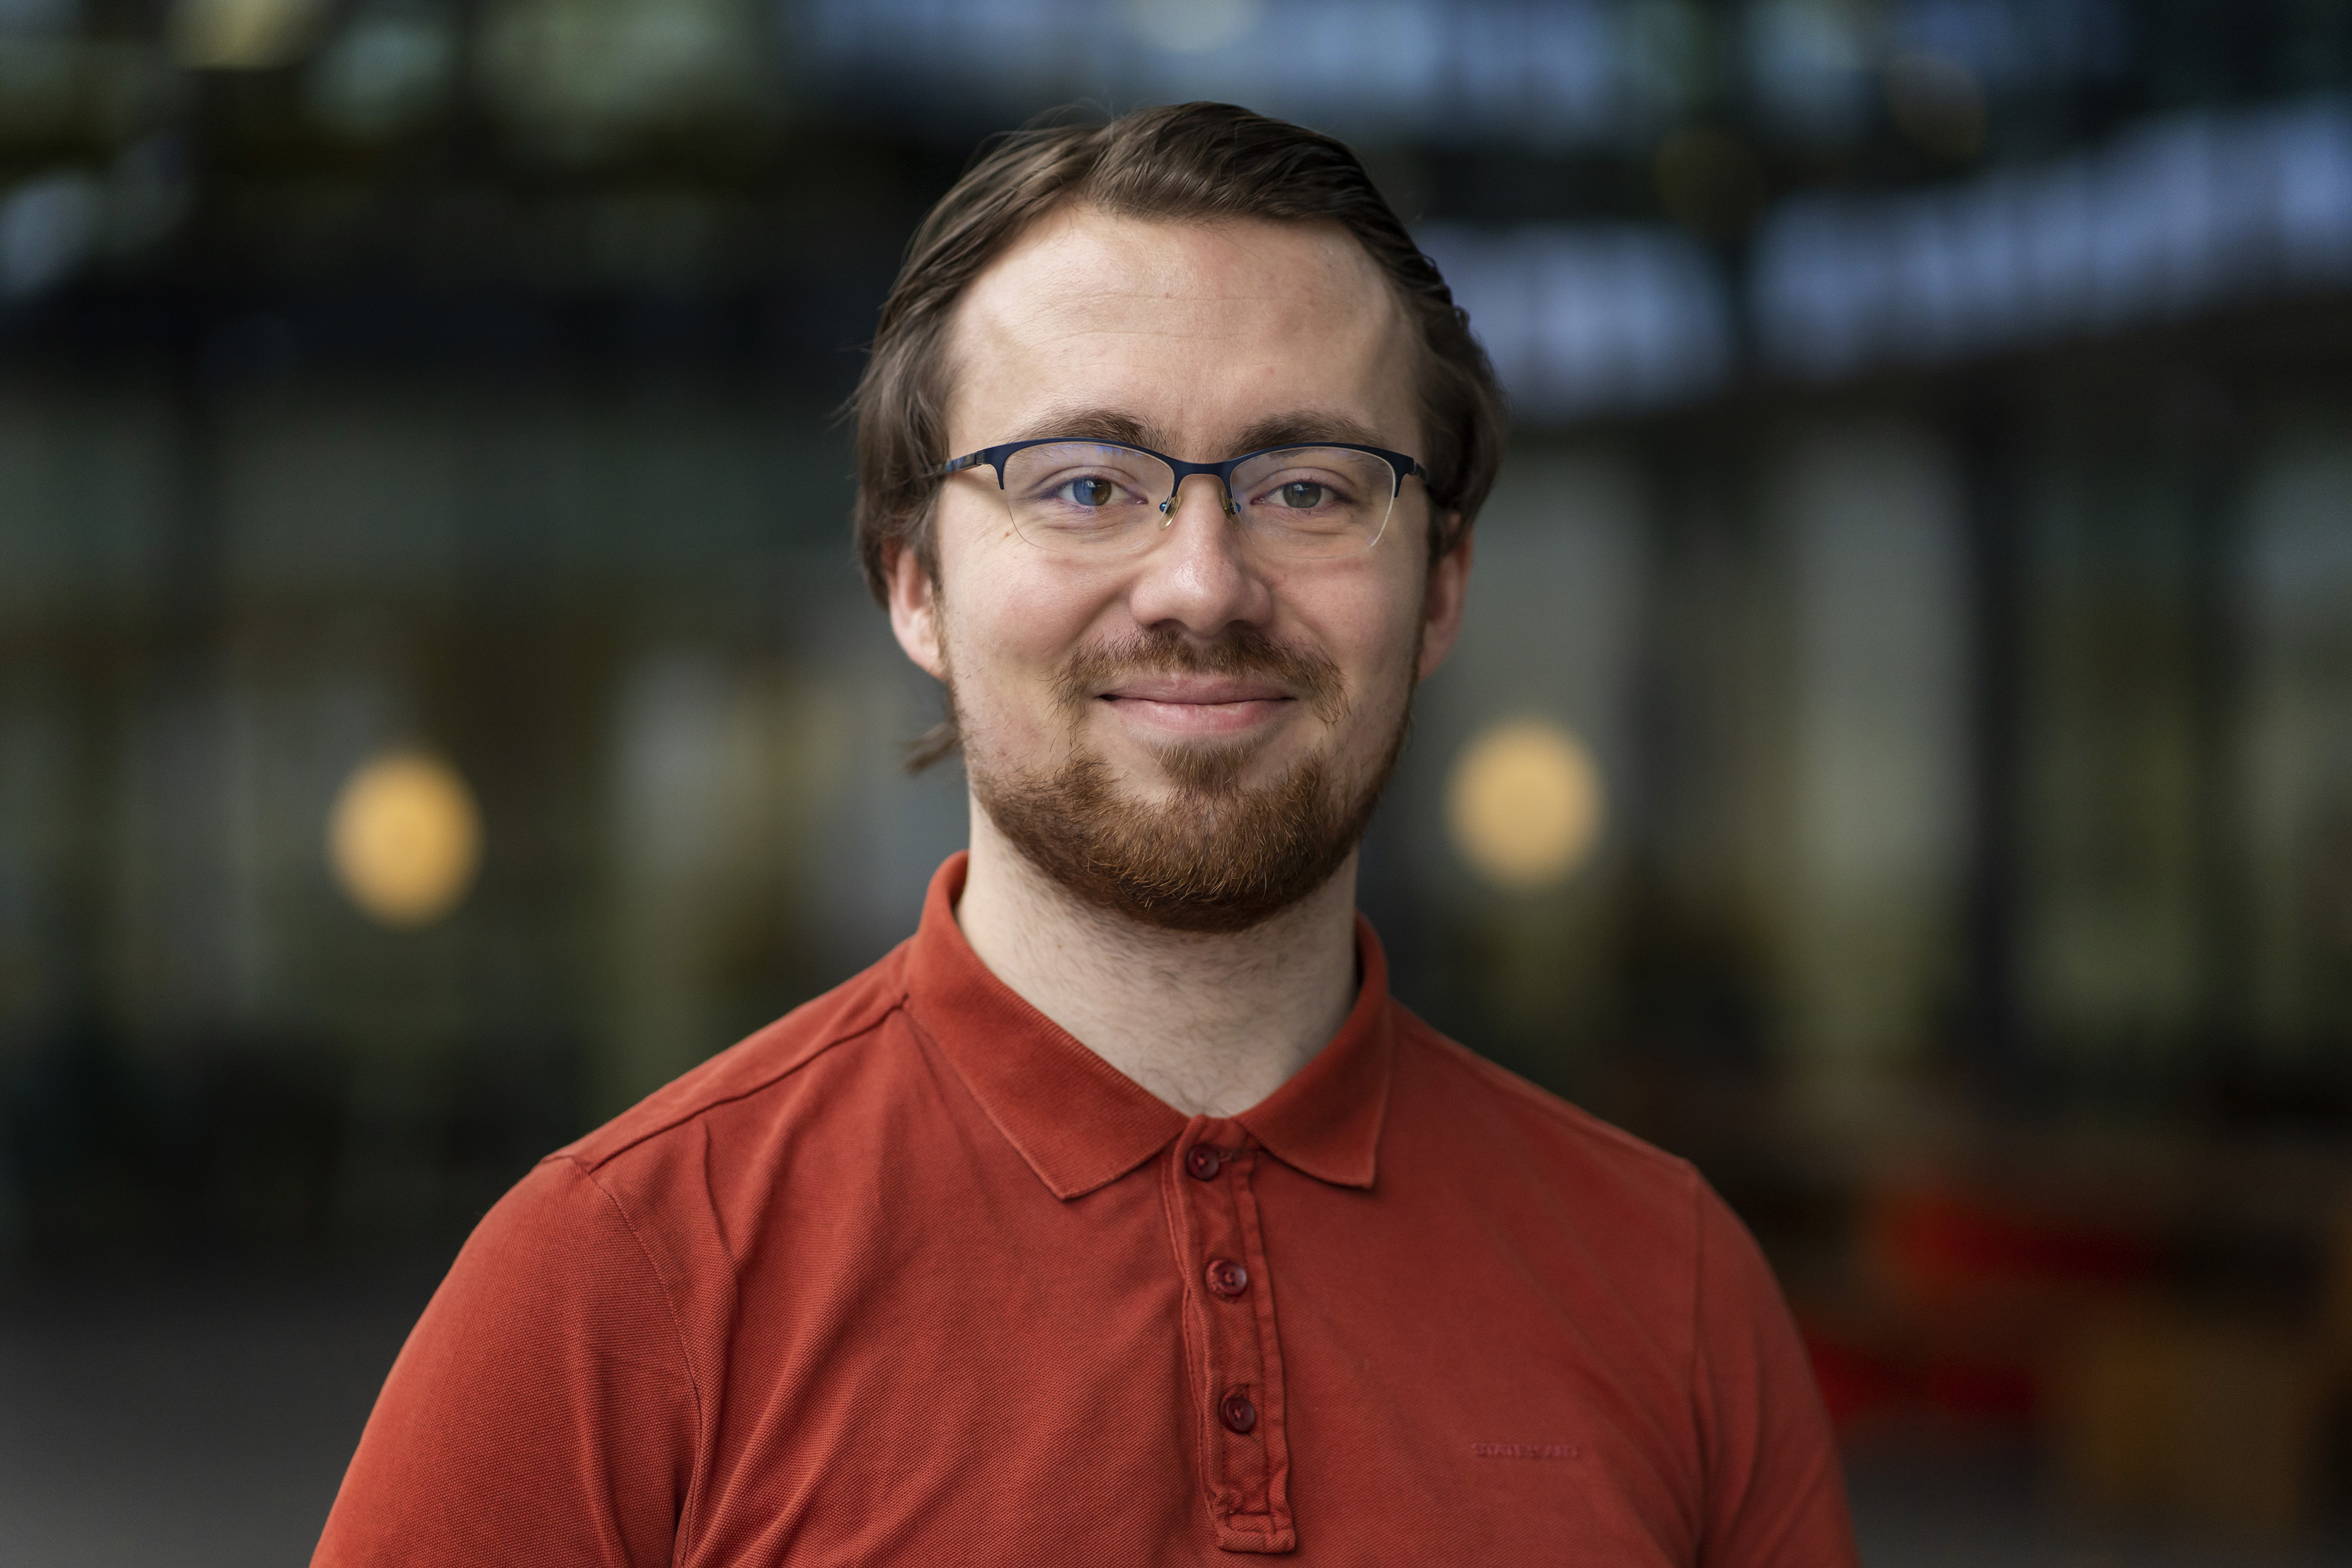
\includegraphics[height=140px, right, trim={4cm 0 6cm 0},clip]{Tom Franken.jpg}
		\end{subfigure}
	\end{figure}
	%\section*{Personal Profile}
	%\section*{Area's of Interest}
	%\begin{itemize}[noitemsep, nolistsep]
	%	\item Algorithms
	%	\begin{itemize}
	%	\item Uncertainty
	%	\item Subtrajectory Clustering/Covering
	%	\item The Fréchet Distance
	%	\end{itemize}
	%	\item Formal Systems Analysis
	%	\begin{itemize}
	%		\item Logic \& Set Theory
	%		\item Algorithms for Model Checking
	%	\end{itemize}
	%\end{itemize}

	
	\section*{Education \& Research Experience}
	\begin{itemize}
		\item \underline{Technical University Eindhoven, PhD Trajectory} \hfill\textit{\color{Blue}{10/2021-current}}
		\begin{itemize}
			\item \textit{Subject}: The Autonomous Data Language: data-autonomous programming with a focus on structure, simplicity, parallelism and verification. Design, Adaptation and the creation of Verification Methods.
			\item \textit{Supervisors}: dr. ir. Thomas Neele (daily supervisor), prof. dr. ir. Jan Friso Groote (main supervisor)
			\item \textit{Side-tracks}: Parallel Algorithms: Adapting Cole's Algorithm, The Expressibility of Switching Graphs  (also known as Binary Parity Games).
			\item \textit{Teaching}: Computer Systems, Practical Tutor\hfill \textit{\color{Blue}{2022-2024}}\\
			\textit{\color{darkgray}{Leading practical sessions and the grading therein, designing exam questions, efforts in further developing the course.}}
		\end{itemize}
		\item \underline{Technical University Eindhoven, Master Computer Science} \hfill \textit{\color{Blue}{09/2018-08/2021}}
		\begin{itemize}[noitemsep, nolistsep]
			%\item Software Science Stream
			\item \emph{Final Project:} \textbf{\href{https://research.tue.nl/en/studentTheses/set-system-oracles-for-subtrajectory-clustering}{Set System Oracles for Subtrajectory Clustering}}
			\begin{itemize}
				\item \emph{Subject}: How to create a data structure to function as a set system oracle for use in solving Subtrajectory Covering with Greedy Set Cover.
				\item \emph{Supervisors}: dr.~Kevin Buchin (TU Eindhoven), prof.~dr.~Anne Driemel (University Bonn).
			\end{itemize}
			%\item Electives: focus on Algorithms \& Formal Systems Analysis Courses
			\item \emph{Internship}:
			\begin{itemize}
				\item \emph{Subject}: Formally translating Hierarchical Equation Systems into Parameterized Boolean Equation Systems and the use of CHC solving on both HES and its equivalent PBES.
				\item \emph{Supervisor}: Tim Willemse (Technical University Eindhoven)
			\end{itemize}
		\end{itemize}
		\item \underline{Technical University Eindhoven, Bachelor Computer Science} \hfill \textit{\color{Blue}{09/2015-07/2018}}
		\begin{itemize}[noitemsep, nolistsep]
			\item Combined Majors Software Science \& Web Science
			%\item \textit{Bachelor End Project:}
			%	\begin{itemize}[noitemsep, nolistsep]
				%		\item The development of the \textbf{Soccer Robot Remote} for Tech United, the autonomous Soccer Robot Team of the TU/e. Includes the development of a frontend with React and styled-components (tested with Jest), a backend with Go and JSON and the production of several official documents and documentation for the Soccer Robot Remote.
				%	\end{itemize}
			%	\item \textit{Electives:}
			%	\begin{itemize}[noitemsep, nolistsep]
				%		\item Courses on Graphics and Artificial Intelligence
				%		\item Courses on Entrepreneurship
				%	\end{itemize}
			\end{itemize}
			\item \underline{Stedelijk Gymnasium Den Bosch (SGDB)} \hfill \textit{\color{Blue}{09/2009-07/2015}}
			\begin{itemize}[noitemsep, nolistsep]
				\item \textit{Profile:} Nature \& Technology and Nature \& Health
			%	\item \textit{Notable Electives:}
			%	\begin{itemize}[noitemsep, nolistsep]
				%		\item German
				%		\item Art/Music
				%		\item Biology
				%		\item Computer Science
			\end{itemize}
		%\item Primary School \hfill \textit{\color{Blue}{$<$07/2009}}
		\end{itemize}
	\section*{Work Experience}
	\begin{itemize}
		\item Student jobs at the Technical University Eindhoven:
		\begin{itemize}[nolistsep]
			\item Student Assistant Logic \& Set Theory\hfill \textit{\color{Blue}{09/2017-10/2017 \& 09/2020-11/2020}}\\
			\textit{\color{darkgray}{Grading weekly tests and assisting at tutor sessions.}}
			\item Student Assistant Algorithms\hfill \textit{\color{Blue}{11/2018-01/2019 \& 09/2019-11/2019}}\\
			\textit{\color{darkgray}{Grading weekly homeworks and assisting at tutorial sessions.}}
			\item Student Assistant Computer Systems\hfill \textit{\color{Blue}{02/2018-04/2018}}\\
			\textit{\color{darkgray}{Grading during tutorial sesions, as well as chat monitoring and answering questions during lectures.}}
		\end{itemize}
	\end{itemize}
	\section*{Other Professional Experiences}
	\begin{itemize}
		\item Treasurer of E.P.A. Nexus \hfill \textit{\color{Blue}{04/2024-current}}\\
		\textit{\color{darkgray}{Bookkeeping and budgeting as a treasurer, also involved in activity planning.}}
		\item Member of the TU/e Math and Computer Science Department PhD Council \hfill \textit{\color{Blue}{10/2022-current}}\\
		\textit{\color{darkgray}{Discussing departmental policies and problems and how they relate to PhDs.}}
		\item Chairman of the Institute for Programming research and Algorithmics PhD Council \hfill \textit{\color{Blue}{06/2022-current}}\\
		\textit{\color{darkgray}{Point of Contact for the IPA director, organising the social event on the IPA Fall Days.}}
				
		%	\textit{\color{Blue}{I assist in the Sunday service. Since recently, I also read certain parts during the service.}}
		%\item Active Member of Da Vinci, Archery Association Eindhoven  \hfill \textit{\color{Blue}{09/2015-now}}
		\item Secretary of Da Vinci, Archery Association Eindhoven \hfill \textit{\color{Blue}{11/2016-10/2017, 10/2020-09/2021}}\\
		\textit{\color{darkgray}{Answering mails, doing member administration, planning activities and making minutes of meetings.}}
		\item Member of Student Team T.E.S.T. (TU/e Sensing Team)\hfill \textit{\color{Blue}{11/2017-09/2018}}\\
		\textit{\color{darkgray}{A student team project to create a biosensor for the SensUs competition.}}
		%		T.E.S.T. is a team competing in the SensUs competition, organized by TU/e students. The goal is to create a biosensor to detect an antibody (which was chosen to be Vancomycin in my year). I have been involved in the market research and the Software and Hardware of the envisioned biosensor.}}
		%\item Saturday machinery cleaning job at a butcher \hfill \textit{\color{Blue}{09/2014-12/2017}}\\
		%	\textit{\color{Blue}{I cleaned two machines, machine parts, plates, cutlery and several other things with specialized tools.}}
		%\item Kitchen Employee at the Jeroen Bosch Hospital, Den Bosch \hfill \textit{\color{Blue}{08/2013, 08/2014}}\\
		%	\textit{\color{darkgray}{I helped with the composition of meals, which meant around 2 or 3 times about 2 or 3 hours of food assembly line work.}}
		%\item Internal Postman at the Jeroen Bosch Hospital, Den Bosch \hfill \textit{\color{Blue}{08/2013}}\\
		%	\textit{\color{Blue}{The job concerned the sorting and delivery of post throughout the hospital.}}
		%\item Member (Keyboard/Piano) of the SGDB School Orchestra, Mercator \& Musica \hfill \textit{\color{Blue}{09/2009-07/2015}}\\
		%	\textit{\color{darkgray}{We made music as an orchestra during the year, the highlight being the Orkestival in the Royal Concertgebouw in Amsterdam.}}
		%\item Participant of several iterations of the Musical (Orchestra) at the SGDB, Den Bosch \hfill \textit{\color{Blue}{09/2010-04/2015}}\\
		%	\textit{\color{darkgray}{I was part of the orchestra and played keys. We were responsible for all musical accompaniment during the performance.}}
		%\item Member of the SGDB Model European Parliament Team\hfill \textit{\color{Blue}{04/2013}}\\
		%	\textit{\color{darkgray}{A week of debating and imitating European Politics, each team with their own goals, suits and real facts. Included several excursions about politics and europe.}}
		%\item Lector at the St. Lambertus Church, Den Bosch \hfill \textit{\color{Blue}{2004-now}}\\
	\end{itemize}
	\renewcommand\labelitemi{$\circ$}
	\section*{Conferences and Reviews}
	\begin{figure}[h]
	\begin{subfigure}[t]{0.5\textwidth}
		\subsection*{Attended}
		\begin{itemize}[noitemsep, nolistsep]
			\item SEFM 2023 \textit{(helper)}
			\item ICTAC 2023 \textit{(accepted paper)}
			\item FORTE 2024 \textit{(accepted paper)}
		\end{itemize}
	\end{subfigure}
	\begin{subfigure}[t]{0.5\textwidth}
		\subsection*{Reviewed for}
		\begin{itemize}[noitemsep, nolistsep]
			\item SETTA 2022 \& 2023 \textit{(subreviewer)}
			\item FMICS 2022 \textit{(subreviewer)}
			\item iFM 2023 \textit{(subreviewer)}
		\end{itemize}
	\end{subfigure}
	\end{figure}
	\section*{Skills and Interests}
	\begin{figure}[h]
		\begin{subfigure}[t]{0.5\textwidth}
			\subsection*{Languages}
			\begin{itemize}[noitemsep, nolistsep]
				\item Dutch, \textit{native language}
				\item English, \textit{fluent}
				\item German, \textit{basic}
				\item Italian, \textit{basic}
			\end{itemize}
		\end{subfigure}
		%\begin{subfigure}[t]{0.5\textwidth}
		%	\vskip 0pt
		%	\subsection*{Programming Languages}
		%	\begin{itemize}[noitemsep]
		%		\item Java, \textit{advanced}
		%		\item Python, \textit{advanced}
		%		\item \LaTeX, \textit{advanced}
		%		\item HTML/CSS/JavaScript \& React, \textit{intermediate}
		%		\item C, \textit{beginner}
		%		\item C++, \textit{beginner}
		%		\item Go, \textit{beginner}
		%		\item JSON, \textit{beginner}
		%		\item SQL, \textit{beginner}
		%		\item Rascal, \textit{beginner}
		%	\end{itemize}
		%\end{subfigure}
		%\begin{subfigure}[t]{0.5\textwidth}
		%	\vskip 10pt
		%	\subsection*{Sports}
		%	\begin{itemize}[noitemsep]
		%		\item Archery
		%		\item Walking
		%		\item Bicycling
		%		\item Swimming
		%		\item Dancing
		%	\end{itemize}
		%\end{subfigure}
		\begin{subfigure}[t]{0.5\textwidth}
			\subsection*{Research Interests}
			\begin{itemize}[noitemsep, nolistsep]
				\item Parallel Verification
				\item Parallel Algorithms
				\item Concurrency
				\item Uncertainty
				\item Graphs \& Games
				\item Parallel Hardware (less developed)
			\end{itemize}
		\end{subfigure}
		\begin{subfigure}[t]{0.5\textwidth}
			\subsection*{Hobbies}
			\begin{itemize}[noitemsep, nolistsep]
				\item Cooking
				\item Board- and Roleplaying Games
				\item Music
				\item Archery
				\item Travel Sports (walking, biking, swimming)
			\end{itemize}
		\end{subfigure}
	\end{figure}
	\section*{Publications}
	\nocite{*}
	\bibliographystyle{splncs04}
	\bibliography{refs.bib}
\end{document}